\documentclass[10pt,a4paper,twocolumn]{article}

\usepackage[top=0.6in]{geometry}

%for links
%\usepackage[hidelinks]{hyperref}
\usepackage{hyperref}

%for bilbiography
\usepackage{natbib}

%for images
\usepackage{graphicx}
\usepackage{caption}
\usepackage{subcaption}

\author{Dionisio Perez-Mavrogenis}
\title{Firmware Protection and Attacks Against the ATMega Microcontroller Series}
\date{\today}

\begin{document}
	\maketitle
	
\section*{\emph{Abstract}}
	\textbf{\emph{The most abstract abstract of some abstracts, full of abstractions.}}
	

\section{Introduction}
	This paper will present an overview of the current attacks and methods of tampering with Intellectual Property (IP) in MicroController Units (MCUs). In this context IP does not solely refer to the firmware running on the MCU but it includes information that could be obtained from that code, i.e. secrets or proprietary algorithms that help a manufacturer achieve higher performance over their competitors.
	
	Tampering (or theft) detection and prevention of the firmware of a MCU is a popular problem with active research, as solving it would benefit a lot of parties (including the government and the military), as MCUs are used in areas spanning from consumer electronics to missile guiding systems.
	
	A distinction between ordinary and secure microcontrollers should be made\citep{website:scorobogatov_breaking_copy_protection} and, due to the sophistication in the protective mechanisms and the attack vectors, a broad classification of attackers as\cite{anderson:cautionary_note}:
		\begin{itemize}
			\item \textbf{Home Hackers} Clever and curious people with a very limited budget, perhaps with some degree of knowledge and no malicious intent, but with no time-limit.\\
			\item \textbf{Semi-Professional Crackers} Professionals skilled on electronics with access to specialised equipment and resources. Their funding might be limited, malicious intent is unclear and they might be constrained in their time allowance.\\
			\item \textbf{Funded Organisations} Organisations with access to MCU manufacturing equipment. Their funding is usually unconstrained, there usually exists malicious intent and their time schedule is usually tight.
		\end{itemize}
	
	Firmware tampering or theft has a number of consequences. The most obvious consequence is an attacker downloading the code from a MCU and flashing it onto a MCU that they sell, effectively avoiding development and testing costs but still offering the same product as other manufacturers(\cite{tech:aes_bls}). A less obvious, but perhaps more important, case is the case of back-dooring\footnote{The act of adding code to a system without the user's knowledge or approval, usually to accomplish nefarious tasks.} a MCU by re-flashing on it a modified version of the firmware with coded added by the attacker in order to accomplish their malicious intents, which could have disastrous consequences if these MCUs were used for military or other sensitive operations. 

	\subsection{Objectives}
	The aims of this paper are to review the possible attacks against the ATmega series of MCUs and provide possible countermeasures or possible methods of hardening a system. 
	
	Section \ref{sec:atmega_overview} will provide an overview of the ATmega series of AVRs and explain the most important hardware architecture aspects and protection mechanisms they offer. 
	
	Section \ref{sec:curr_attacks} will give a (brief) overview of the current attack techniques used to override currently implemented protection mechanisms, an overview of whom is given in Section \ref{sec:defenses}. 
	
	In section \ref{sec:attacking_mega} the current attacks will be related to the ATmega, by presenting the attack vectors in more detail as well as providing references to relevant work. Section \ref{sec:conclusion} will conclude the paper with a discussion on the usefulness of hardening the ATmega, contrasting that with using a MCU that is designed to be secure.
	
\section{The AVR MCU Series}
\label{sec:atmega_overview}

	The Atmel AVR series is an enhanced-RISC MCU family that consists of the ATtiny, ATmega and ATxmega sub-categories and derivatives of the above, including 32-bit AVRs and application specific FPGAs\footnote{info:\href{http://www.atmel.com/products/microcontrollers/avr/default.aspx}{AVR family link}}. The models have varying degrees of hardware capabilities and large operating voltage windows in order to accommodate demand and integrate well with peripherals\footnote{info:\href{https://www.newbiehack.com/MicrocontrollersAlternativePowerSources.aspx}{https://www.newbiehack.com}}\footnote{info:\href{http://www.atmel.com/v2PFResults.aspx}{http://www.atmel.com/v2PFResults.aspx}}.
	
	Developing software for an AVR is easy as the AVRs benefit from the free \texttt{avr-libc} high-performance C run-time library(optimised for the AVR RISC architecture), the \texttt{avr-gcc} and \texttt{avr-gdb} compiler and debugger(both based on very popular and high quality GNU software tools), the \texttt{avrdude} programming software(or Atmel's proprietary \texttt{AVRStudio}) and \texttt{Simulavr} simulator software. Additionally, Atmel provides proprietary APIs for interacting with the AVR and the developers can choose from a wide variety of programmer units available for working with the AVRs\cite{book:practical_avr}.
	
	\subsection{ATMega Architecture and Features}				

	\subsubsection{Important Feature Overview}
	The ATmega series of MCUs is a relatively large family of MCUs and the focus of this paper is on the ATmega644 and ATmega1284. The only differences between then 1284 and the 644 is that the 1284 has got more memory available and an hardware extra timer. A summary of (some) of the features of the two units is give in Table \ref{table:avr_specs}\citep{atmega_manual}. 
	
	Both MCUs are an enhanced-RISC Harvard architecture 8-bit CPU. Figure \ref{fig:architectures} shows the conceptual difference between a Von Neuman (most modern PCs) and a Harvard architecture, where the key distinction lies in the separation of application code and program data into different memory sections (Harvard) and tasking the CPU with distinguishing between code and data that lives in the same memory region (Von Neuman). The 644/1284 implement a Harvard architecture for both power and computational efficiency, being designed to access more than one registers simultaneously (due to the physical wiring of the CPU), enabling them to execute an instruction per cycle. Their operating voltages can vary between 1.8V and 5.5V (maximum operating frequency 20 MHz).
	
	\subsubsection{Memory Organisation}
	The 644/1284 are equipped with an EEPROM, flash memory, SRAM, a large number of general purpose registers and a large number of I/O registers (in order to be able to perform I/O) and all memory (including I/O memory mapped images) is linear, i.e. it follows the flat memory model.
	
	The flash memory is separated into two regions, the bootloader section and application code section. The boundary between the two sections can be configured by programming the appropriate fuses, and the page size can also be configured that way as well. Both sections hold code, however code residing in the bootloader section can execute a special instruction (\texttt{SPM}\footnote{\texttt{SPM} = Store Program Code}) which allows the bootloader code to write to \textit{any} section in the flash memory and hence possibly modify itself(designed for purposes such as firmware upgrades). The bootloader code can be triggered by a direct jump from the application section or by programming the reset vector via the reset fuse to point to the appropriate section of the bootloader code. 
	
	The EEPROM is memory for data that needs to persist between reboots of the MCU and hence it is (widely) used to hold configuration variables and other non-temporary preferences the application code (or the bootloader) may need, having an average lifespan is 100,000 write cycles per page. 
	
	The SRAM is volatile storage and is used as the stack and heap for the software (either application code or bootloader code) as well as for storing the Register File (i.e. the 32 GP registers) I/O and Extended I/O Memory. The reserved register locations exist in order to support the use of peripheral units as well as hold program status information (e.g. the Stack Pointer can be found in one of the GP registers).Figure \ref{fig:stack} gives an overview of the SRAM hierarchy, which is slightly different (in terms of region sizes) for the 644 and the 1284 as the 1284 offers more SRAM.
	
	\begin{figure}
		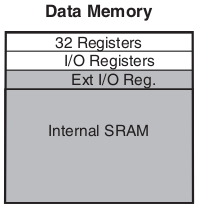
\includegraphics[scale=0.7]{img/stack.png}
		\caption{SRAM layout for the ATmega 644 and 1284. \textbf{Source}:\protect\citep{atmega_manual}.}
		\label{fig:stack}		
	\end{figure}
	
\begin{figure*}
	\begin{subfigure}{0.5\textwidth}
		\center
		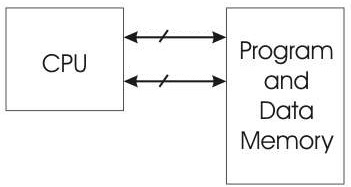
\includegraphics[scale=0.5]{img/von_neuman_arch.jpg}
		\caption{Schematic of a Von Neuman architecture.}
		\label{fig:VN_arch}
	\end{subfigure} 
	~
	\begin{subfigure}{0.5\textwidth}
		\center
		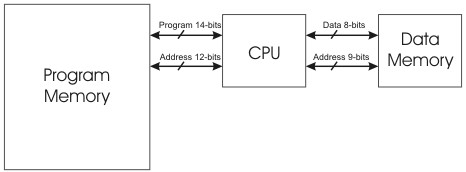
\includegraphics[scale=0.5]{img/harvard_arch.jpeg}
		\caption{Schematic of a Harvard architecture.}
		\label{fig:H_arch}
	\end{subfigure}
	\caption{A comparison of different machine architectures. \textbf{Source}:\protect\citep{website:mcu_primer}.}
	\label{fig:architectures}
\end{figure*}	
		
\begin{table*}
	\begin{tabular}{| c | p{2cm} | p{1.5cm} | p{1.5cm} | p{2.8cm} | p{1.9cm} |}
		\textbf{Model} & \textbf{EEPROM (Kb)} & \textbf{SRAM (Kb)} & \textbf{Flash (Kb)} & \textbf{JTAG Interface}\\
		ATmega644 & 2 & 4 & 64 & Yes\\
		ATmega1284 & 4 & 16 & 128 & Yes \\
	\end{tabular}
	\caption{Specification overview for the AVR ATmega644 and ATmega1284}
	\label{table:avr_specs}
\end{table*}
	
	\subsection{ATMega Security Features}
	
	The AVR ATmega644/1284, even though not meant to be secure hardware modules, posses certain security features. In particular, each board provides six Lock bits responsible for controlling access to the board's memory and prevent reading or modifying the memory (e.g. prevent code executing from the bootloader section to read/write the application code section via the \texttt{SPM} instruction). This access control is not permanent, as that would limit the usefulness of the MCU and therefore one has the option to reset the lock bits (i.e. having no protection scheme enabled) by issuing a Chip Erase command, which has the effect of completely erasing the Flash, EEPROM and Lock bits.
	
	The erasing is performed with the sequence of events presented above and this is important, as one does not want to remove the access protection before removing all sensitive data and hence the Lock bits are set to 1 only after the whole program memory has been erased. Even though the flash memory has an average lifespan of 10,000 write cycles (as well as programming being relatively expensive as an operation) this approach makes sense as the ultimate goal is to preserve the intellectual property on the board rather than the board itself.
	
	\begin{table}
		\center
		\begin{tabular}{| c | c | c | c |}
			\hline
			\textbf{Lock Bit Byte} & \textbf{Bit Number} & \textbf{Default}\\
			\hline \hline
			BLB12 & 5 & 1\\
			BLB11 & 4 & 1\\
			BLB02 & 3 & 1\\
			BLB01 & 2 & 1\\
			LB2 & 2 & 1 \\
			LB1 & 1 & 1 \\
			\hline
		\end{tabular}
		\caption{Security lock bits offered by the ATmega644 and ATmega1284. BLB stands for Boot Lock Bit and LB for Lock Bit.}
		\label{table:lock_bits}
	\end{table}
	
Table \ref{table:lock_bits}	 provides an outline of the available Lock bits provided by the ATmega series. The functionality of the BLB1 group is to control access and modification of the bootloader section, group BLB0 bits control access to the application code section and group LB bits are responsible for controlling modifications on the EEPROM and Flash.A detailed explanation of their functionality and how to use them is given in \citep{atmega_manual}.
	
\section{Attacks on Hardware}
\label{sec:curr_attacks}
A distinction between \emph{passive} and \emph{active} attacks should be made. In the former the attacker simply monitors the chip's normal operation and tries to infer the input-output mapping whereas in the latter case the attacker actively manipulates either the chip or its operating environment with the aim of obtaining insight on the chips inner workings. 

Attacks on MCUs may attempt to recover a number of artefacts, including cryptographic keys from the flash or the EEPROM or read the firmware off the flash and do not need to necessarily attack the hardware itself but can exploit flaws in algorithmic design and implementation and protocol failures or inter-component communication patterns\citep{anderson:cautionary_note}\citep{kocher:DPA}.

[REWRITE THIS BIT/GATHER MORE INFO]obtain information by corrupting the memory or exploiting memory remanence\citep{sergei:thesis}.
	\subsection{Non-Invasive Attacks}
	Non-invasive attacks are attacks which require no de-packaging or special preparation of the chip and hence attacks under this category leave little tamper evidence behind. These attacks might be very time consuming and are not guaranteed to be successful, but are very easy and cheap to replicate once found. Furthermore, non-invasive attacks could target badly implemented communication or security protocols in order to bypass security restrictions.
	
	\subsubsection{Power Analysis}
	\label{subsubsec:power_analysis}
	Different instructions executing on a CPU require different amounts of power, and hence one can infer which instruction is executing on a CPU by constructing and analysing a power trace generated by the MCU's operations. These attacks are easy and relatively inexpensive to perform as they only require widely available tools.
	
	Simple Power Analysis(SPA) involves direct observation of the MCU when it performs cryptographic operations and can leak information about both the keys and the cryptographic operations themselves (i.e. nature or structure of the algorithm). 
	SPA-DPA
	\subsubsection{Glitch Attacks}
	power/clock glitch attacks
	\subsubsection{Data Remanence}
	Data remanence \citep{anderson:tamper_resistance}\citep{gutman:memory_remanence},
	\subsubsection{Timing Attacks}
	Timing attacks are possible because of the software implementation of cryptographic algorithms, where compiler optimisations (avoiding unnecessary branches, register and cache usage) and other implementation choices make the execution time of an algorithm dependent on the input and the secret key, rather than having a fixed time for every key. A characteristic example would be when an input is compared byte-wise with a key and rejected when the first non-matching byte is found, rather than first consuming the whole input string.
	
	Different instructions take different time to execute(e.g. \texttt{MOV eax,[eax]} is considerably slower than \texttt{INC eax}) and thus one could collect timing information on various input messages and systematically deduce the correct key. 
	
	If timing information is correlated with power analysis then defences such as constant instruction execution time could be defeated. For example, one might use \texttt{NOP}s in the case of a wrong key in order for rejection and confirmation responses to have constant execution time. However, \texttt{NOP} would consume substantially less power than \texttt{INC eax} and hence correlating timing and power consumption information could prove dangerous.

	\subsection{Semi-Invasive Attacks}
	some sort of fault injection?
		all memory types are linear( as well as memory mapped IO) - related to memory scanning attacks by glitching and power faults (stop making call or jump instructions)
	\subsection{Invasive Attacks}
	mention decaping and chip exposure. can be done by sending to hardware failure test labs\citep{website:hacking_the_pic} or by chemicals etc \citep{anderson:cautionary_note}
	Microprobing
	overview of attack categories [each one to the category that it corresponds above]
	\begin{itemize}
		\item microprobing \\
		\item side-channel attacks \\
		\item software attacks (exploit communication protocols or crypto implementation and such) \\
		\item reverse engineering of hardware\\
		\item fault generation (power/clock glitches ) \\
	\end{itemize}
	
	* for each category discuss budget/tools/skillset/time required\\

\section{Countermeasures to known attacks}
\label{sec:defenses}

As demonstrated in the previous section a manufacturer has to guard against a multitude of attacks. For designing effective defensive mechanisms one has to enumerate the likely attack scenarios and methods, type of attacker they will be facing and decide the type and extend of confidentiality they would like to provide\citep{sergei:thesis}.

A common first line of defense that is often encountered in attempts to secure systems, with questionable effectiveness, is security by obscurity and in the case of MCUs can be achieved in a number of different ways. As a starting point, the manufacturers can simply avoid printing their logos or model numbers on parts they produce, as this will make information gathering for he chip trickier. Some vendors take this even further by printing on their products identifiers of more secure or expensive products \footnote{Related legal issues discussed in Sec.~\ref{sec:conclussion}\red{hardware reveng legal issues}} or even try to make their MCUs look like ASICs \red{abbreviation?} in order to scare away potential attackers by making their product appear more secure\citep{sergei:thesis}. A further step in making the MCU harder to analyze is hardware obfuscation, where a group of gates commonly placed in well known structures for performing a given task (for example DES circuitry) is intentionally made more complicated and physically placed in a different locations or additional circuitry is added in order to thwart analysis\citep{anderson:cautionary_note}. Vendors also try to make information on their products hard to find by selling only to selected partners or under non-disclosure agreements\citep{sergei:thesis}.

Security through obscurity has received lots of criticism, and rightfully so, as it will do little to stop experienced or determined attackers. Despite its financial appeal a more effective approach is security in depth, a model in which information is protected by a number of (potentially) different defense mechanisms and in this scenario could be employed at different levels of the chip, from its external potting (or encasing) to its layered architecture. Given the attack categories presented in Sec.~\ref{sec:curr_attacks}, it would be useful to broadly categorize denfences in a similar fashion.

Non-invasive attacks are the least sophisticated type of attack but protection against them is a relatively laborious process\citep{anderson:cautionary_note}. To start with, one has to mask all the side-channel leakage and this means mask all relationships between data input and power consumption, thermal and electromagnetic radiation and timing relationships\citep{kocher:DPA}\cite{sergei:thesis}. Given the software release model and the power of MCUs it's not unreasonable to strive for efficiency, both in terms of power and components. Bytecode optimizations performed by compilers and the hardware architecture of the instruction pipeline of an MCU might introduce leakage potential \citep{kocher:DPA}\citep{sergei:thesis} by how branches are taken, instructions pre-fetched or not take constant time for operations. Even if constant time is taken for correct and erroneous keys such that timing relationships are masked, intermediate result storage is still a problem due to the fact that a 0 and a 1 consume different power when handled (due to the physical nature of CMOS transistors) and hence the power consumed in a given operation is proportional to the amount of 1 bits, a concept known as "Humming weight"\citep{website:riscure}\citep{kocher:DPA}\red{maybe read this about CPA as well https://www.iacr.org/archive/ches2004/31560016/31560016.pdf }. Electromagnetic or thermal emission detection can be avoided by packaging that is appropriately shielded\red{reference needed}. \red{also destroying circuitry and lock bits}

also have self health tests to detect alteration\citep{anderson:tamper_resistance}

Protection against invasive and non-invasive attacks is a lot harder because these attacks involve a range of chip modifications (from decapsulation to modification of the die), requiring varied anti-tampering mechanisms; we will proceed to give a description in the order in which decapsulation occurs. Thwarting decapsulation can get very creating as it is dependent on the material from which the chip packaging is made from. tries In order to protect from semi-invasive attacks (such as exposure to radiation or optical inspection
\subsection{Physical Protection}
asic glue logic design, protective metal-mesh layer, shrink things, mesh of wires, encase in epoxy, make layers destroy each other if removed. doping can also reduce light penetration to reduce imaging attacks 
\subsubsection{Protection circuits}
radiation/temperature/voltage/frequency detector circuits that cause reset on abnormality detection (instability reference \citep{anderson:cautionary_note}). add transistors on top to hide true signal (provide reference)
 keep keys in own, self powered module.
\subsection{Side-channel Protection}
decrease signal/noise ratio (either by introducing noise or making the signal smaller), constant time/power operatations, insert random delays\citep{sergei:thesis}, \citep{kocher:DPA} and shielding the device.

Planarization defeats optical inspection with microscope (source: Introduction to hardware security and trust, sergei skorobogatov paper).\\
	\begin{itemize}
	\item overview of most popular techniques \\
	\item benefits and how they improve the situation/approach the problem
	\item added cost for this investment (in terms of hardware and money, transparency to the developers, runtime overhead etc)\\
	\end{itemize}
	
	perhaps review some popular secure chips ?? IBM 4758 is a secure device \footnote{\href{http://www.cl.cam.ac.uk/~rnc1/descrack/ibm4758.html}{http://www.cl.cam.ac.uk/~rnc1/descrack/ibm4758.html}}, some Dallas chips and perhaps more.
	
	thermally enhanced packaging : makes difficult to microprobe chips as they need to be cooled or they'll fry [slides of hardware reveng module] and careful decaping needed
	
	ceramic packaging (Al2O3 is common, often mixed with SiO2, AlN and BeO) is extremely chemical resistant and seals very good, but can crack
	
	potting : protects board from environment[water/dirt] but might also make tampering harder and may need to be removed
	conformal coating : same deal as potting, but it's a thin layer that doesn't fill the enclosure but just covers the top.
	underfill : provides stability but gets in the way as well(makes desoldering harder).
\section{Attacking The ATmega}
\label{sec:attacking_mega}

In this section we present the suggested attack that should work against the ATmega644. We believe that someone with a modest level of competence in electronics could successfully bypass the security fuse and lock-bit protections on the ATmega644 board, as researches have succeeded in bypassing the protection imposed by the AVR family in numerous ways. All researches used non-invasive attacks in order to achieve this since there is no need for more sophisticated attacks.Clock glitch attacks against AVR chips were successfully applied by \citep{glitches_paper} against an ATmega163 and by \citep{chipwhisperer} against an ATmega328P and \citep{avr_mega} managed to retrieve AES and DES cryptographic keys from an ATmega16 and ATXmega128A1. Furthermore, \citep{sergei:thesis} also points out that AVR MCUs are susceptible to glitch attacks due to the implementation of their security fuses. 

The suggested attack method will closely follow \citep{glitches_paper}, further supported by results from other research as well. We will be a Class-I attacker performing a non-invasive clock-glitch attack on an ATmega644-based product. The equipment we should have access should be found in any descent university's electronics laboratory and our information regarding the chip will come from datasheets. We believe that the attack engineered by \citep{glitches_paper} on the ATmega163 can be ported over to the ATmega644 due to their similarities. Both devices belong to the same family and by comparing their datasheets we can see that the 744 possesses all the hardware features that make the attack possible on the 163, namely it operates on an external clock signal and has a two stage pipeline. Furthermore, the two devices have an almost identical instruction set.\\

The attack should be tailored to a particular goal and hence we should distinguish the task of recovering cryptographic material from the task of making the device output its memory contents or execute code other than it was intended to, e.g. skipping instructions or executing other instructions. In both cases monitoring the device's power consumption will help us gain some insight into what the device is doing, like in Fig.~\ref{fig:des_power}, and will furthermore allow us to synchronize with the device's operations \citep{sergei:thesis}\citep{avr_mega}. 



might be hard to sync with internal clock


\red{mention service that breaks chips. mention ChipWhisperer paper. perhaps mention pipeline/give examples of clock glitch. mention that no paper found targeting these devices. \citep{glitches_paper} this guy breaks and \citep{sergei:thesis} and website of chinese dude that break atmels.}
\section{Evaluation}
\label{sec:conclusion}

No system is unbreakable and one can only harden their system enough to make the effort of breaking it unbearable to those they wish to protect against\citep{anderson:cautionary_note}\cite{sergei:thesis}.

security is hard to do because one must carefully analyse and model all threas \citep{kocher:DPA}
	not sure if the subsections are needed here
	\subsection{Securing the mega}
		paragraph talking about why it's not a good idea to salvage the mega.
	\subsection{Attacks and Solutions overview}
	\subsection{Conclusions}
	
	\bibliographystyle{plain}
	\bibliography{irp_report}	
	
\end{document}
